\chapter{DDD.jl: next-Gen 3D discrete dislocation dynamics}
\label{c:DDDjl}

During the course of this project, it became increasingly clear there are some fundamental issues preventing us from exploring the full breadth of what discrete dislocation dynamics has to offer. \href{http://micro.stanford.edu/wiki/M01_How_to_Obtain_and_Run_DDLab}{DDLab} \cite{ddlab}, the code that EasyDD is based on, made some design decisions that ultimately limit its potential. Namely, the lack of attention paid to the cost of dynamic memory allocation, procedural nature of the code, and choice of programming language. These choices were reasonable upon inception, but as the Tarleton group has increased in size and maturity, it has become evident that it is not enough. We are reaching the upper limits of what can be done with \mintinline{matlab}{MATLAB}. There are more things we can do, more things we are doing. But a constant obstacle in obtaining results is how long they take to get and how difficult it is to add new functionality, even changing boundary conditions presents a non-trivial obstacle that requires intimate knowledge of how the finite element mesh is generated.

The work described in \cref{c:easydd,c:topology,c:tractions} has done much in not only producing more accurate simulations, but doing so faster. Fengxian Liu's work on modelling climb, diffusion and inclusions would greatly benefit from better designed code. Haiyang Yu's work on modelling hydrogen \cite{YU2018} and nanoindentation would also stand to benefit a great deal from a parallelised and faster dislocation separation algorithm. Potential work relevant to modelling dislocation dynamics in nuclear reactors such as post-damage cascade dislocation dynamics \cite{sand2014radiation}, necessitates spontaneous generation of dislocations as a network evolves. Including stochasticity in the form of Langevin dynamics \cite{li2019diffusion} is also highly relevant, especially at higher temperatures.

Many of these require a complete overhaul to some of the most fundamental parts of EasyDD. Even so, its potential would be hindered by the fact that \mintinline{matlab}{MATLAB} is a scripting language not designed for scientific computing. It lacks performance, flexibility and many of the modern features that make life easy when dealing with large codebases. Furthermore, the need for licences can represent a prohibitative barrier for users and researchers. Not only this, but the cost of distributed licences that allow \mintinline{matlab}{MATLAB} to run on clusters severely limits scalability and potential for collaboration---something that at one point, inhibited this project.

But there is a better way. Prompted by the public release of the Imperial College COVID-19 source code \href{https://github.com/mrc-ide/covid-sim}{\texttt{https://github.com/mrc-ide/covid-sim}}, and the recurring issues with computational efficiency, compiler compatibility and availability, and fundamental technical debt inherited from \texttt{DDLab} \cite{ddlab}. We started a weekend project that has turned out to be \emph{extremely} promising.

It is our belief that we are currently in a renaissance of programming languages. There are so many exciting modern languages that build and improve upon the lessons of the past. The most promising for scientific computing is widely regarded to be \mintinline{julia}{Julia} \cite{julia}. A paradigm-shifting, open-source JIT (just in time) compiled\footnote{Although as of \texttt{v1.6}, it might be more appropriate to say call \mintinline{julia}{Julia} a JAOT (Just Ahead Of Time) compiled language thanks to its massively improved precompilation capabilities.} language, explicitly designed for scientific computing. It has a number of features that make it an excellent candidate for a new generation of scientific software.
\begin{enumerate}
    \item Multiple dispatch: methods are dispatched and compiled based on the types of their arguments. Types propagate their way through child functions. This lets the compiler generate optimal code for the platform being used.
    \item Type system: its type system is based on set theory, where types are arranged in a genealogical tree with broader types giving way to narrower ones, e.g. \mintinline{julia}{Float64 <: AbstractFloat <: Real <: Number <: Any == true}. Structures can be parametric on type. These features let developers create generic code without bothering with type annotations, and the behaviour will be appropriate for whatever types are used. This kind of code greatly improves modularity and allows for ``magic'' such as automatic differentiation by only defining the basic arithmetic rules for dual numbers. It also allows for zero-cost abstractions, letting users represent mathematical equations as they are written without incurring a performance cost.
    \item CPU and GPU Parallelisation: parallelising loops is trivial. The \href{https://llvm.org/}{\texttt{LLVM}} compiler is platform-agnostic and creates custom, optimal code for almost all CPU and GPU architectures. This means users get platform-specific optimisations for free, and it means the software can remain a single language with no detriment.
    \item Metaprogramming: one of the most powerful and esoteric features of \mintinline{julia}{Julia}. Much like \mintinline{lisp}{Lisp}, code is an object that can be manipulated by the language itself. This allows code to write and modify code. This can be used to autoparallelise functions on different architectures without rewriting. It lets developers precompute values like an extremely powerful C-preprocessor. It even lets developers design custom syntax and perform mathematical transformations on code itself, such as symbolic and automatic differentiation.
    \item Modern features: \mintinline{julia}{Julia} has all the features of a modern programming language. From a booming and quickly growing fully-integrated package ecosystem with standard and registered libraries, some of which are now best in class. Integrated testing and documentation generation systems. Extremely powerful code introspection tools, e.g. one can check type stability, call trees, and different stages of compilation all the way down to machine instructions. It also has unicode support and sports all the interactivity and useability of modern interpreted languages.
    \item Interoperability: calling other languages from \mintinline{julia}{Julia} is seamless, so the use of external libraries or languages is as easy as calling a \mintinline{julia}{Julia} function. However, \mintinline{julia}{Julia} is so powerful and performant that most of its packages are single-language. A feature often shared by other modern languages such as \mintinline{go}{Go}, \mintinline{rust}{Rust}, \mintinline{swift}{Swift} and \mintinline{elixir}{Elixir}.
\end{enumerate}

The code can be found here \href{https://github.com/dcelisgarza/DDD.jl}{\texttt{https://github.com/dcelisgarza/DDD.jl}}. Of note are the banners at the top of the README, from left to right they link to
\begin{inparaenum}
    \item the documentation;
    \item automated, remote testing;
    \item two test coverage reports i.e. which lines of code have been hit during testing and how many times; and
    \item an interactive Jupyter notebook on Binder, which runs on a browser and has no external dependancies.
\end{inparaenum}

It is the result of the lessons learned while working on EasyDD. Its design avoids the same pitfalls and has a clear vision for usability, modularity, and extensibility, without sacrificing performance. It has been a didactic, after hours project to escape the anxieties of the pandemic and ease the frustrations with some fundamental design aspects of EasyDD (many carried over from DDLab). But it has also been an attempt to understand how EasyDD can be improved without all the clutter, risk, and technical debt (some solutions were even trialed in DDD.jl and backported to EasyDD). It is therefore not feature-complete. Nevertheless, it has turned into a promising weekend project for which we can provide a sample of current capabilities.

\section{Parameter definition}

As with every simulation, there are parameters that need to be defined. For dislocation plasticity simulations, the number of parameters is quite large, which is why encapsulation (see \cref{ss:encapsulation}) can be so helpful. However, there are also certain relationships between parameters that must be maintained. This is a problem for usability, as it is very easy for one to use non-sensical parameters and be completely unaware of it until a simulation presents unexpected behaviour. We have ``solved'' this issue in EasyDD (see \cref{ss:qol}), but it is clunky, unelegant and opaque. Here we solve both issues in a single stroke and offer greater flexibility.

Setting up simulations is quite easy and there are multiple options.
\begin{enumerate}
    \item Load the data from external files generated by any file extension supported by the \mintinline{julia}{FileIO} ecosystem. In some cases the loaded data has to be used to manually create the structures, but if \mintinline{julia}{JLD2} is used, it works like \mintinline{matlab}{MATLAB}'s \mintinline{matlab}{save()} and \mintinline{matlab}{load()}. JLD2 is advantageous because it saves structure information so loaded variables will be of the correct type, however it is specific to \mintinline{julia}{Julia} and is still under active development.
    \item Use the built-in serialiser. This works like \mintinline{matlab}{MATLAB}'s built-in \mintinline{matlab}{save()} and \mintinline{matlab}{load()} functions. This is another great option that is in-built to the language, but is also \mintinline{julia}{Julia}-specific and successfully reading files is only guaranteed if they were generated with the same version of \mintinline{julia}{Julia} being used.
    \item Use the specially defined functions that load \mintinline{java}{JSON}\footnote{\mintinline{java}{JSON} is an open standard for representing objects as dictionaries in a file. It is widely used by web develpers because it is language agnostic, has high compressibility ratios, and is human-readable.} files and create the structures automatically. Since \mintinline{java}{JSON} is a human-readable format, this is the preferred method for creating sets of parameters that can be used in multiple simulations and loaded from the same file. It is also quite advantageous for sharing data because they have high compressibility ratios and anyone can open a JSON file to have a look at the data. We have internal functions that validate the data and initialise the structures from these files. However, any changes made to the data structures must be accounted for in the IO functions.
    \item Create the structures manually. This can be done by directly using the structure constructors or by using the keyword constructors. When manually creating the variables, using the keyword functions is preferred as they perform validations, calculate derived values, and provide sensible defaults.
\end{enumerate}

Here we show how easy it is to manually set up a simulation. We have to start by defining our parameters.

Almost all of our keyword constructor functions provide default values in case the user does not provide them. They also perform validations on the data to ensure it is sensible, for example the maximum length of a dislocation line must be larger than the minimum length. For demonstration purposes, we provide some values and let the code figure out the rest from what we gave it. This means function signatures can be even shorter than what is shown here.
\begin{minted}[frame=lines, linenos]{julia}
# Dislocation parameters
dlnParams = DislocationParameters(;
    mobility = mobBCC(),
    dragCoeffs = (edge = 1, screw = 1e-1, climb = 1e9, line = 1e-5),
    coreRad = 0.015 * sqrt(2),
    minSegLen = 0.15 * sqrt(2),
    maxSegLen = 1.5 * sqrt(2),
    coreEnergy = 1 / (4 * π) * log(0.015 * sqrt(2) / 3.5e-5),
    coreRadMag = 3.5e-4
)
# Material parameters
matParams = MaterialParameters(;
    crystalStruct = BCC(), μ = 1, μMag = 80e3, ν = 0.25
)
# FEM parameters for a regular cuboid mesh with linear elements
# with the purpose of modelling a cantilever loading experiment
femParamsC = FEMParameters(;
    type = DispatchRegularCuboidMesh(),
    order = LinearElement(),
    model = CantileverLoad(),
    dx = 23.0, # Length in x
    dy = 17.0, # Length in y
    dz = 13.0, # Length in z
    mx = 7, # Elements in x
    my = 5, # Elements in y
    mz = 3  # Elements in z
)
# Slip system information for two BCC slip systems
slipSystems = SlipSystem(;
    crystalStruct = BCC(),
    slipPlane = Float64[-1 1; 1 -1; 0 0],
    bVec = Float64[1 1; 1 1; 1 -1]
)
# Integration parameters
intParams = IntegrationParameters(;
    method = AdaptiveEulerTrapezoid(),
    abstol = dlnParams.collisionDist / 2,
    reltol = dlnParams.collisionDist / 2
)
# Integration time variables
intTime = IntegrationTime(; dt = 0.0, time = 0.0);
\end{minted}
All together, these represent about 60 constants that control all aspects of a simulation. But we're only just getting started.

\mintinline{julia}{Julia} is a fully compiled language, where files can be run from a terminal like any other compiled language. But because it is JIT-compiled, we can ask it questions about our variables, types, functions, etc.\footnote{We represent interactive REPL (Read Eval Print Loop, i.e. \mintinline{julia}{Julia}'s ``terminal''), use by omitting line numbers. Moreover, the \LaTeX{} package, \texttt{minted}, does not accurately represent REPLs so the syntax highlighting will be off in these cases. Regardless, \mintinline{julia}{Julia} uses Markdown natively, so it produces documentation and answers such queries in Markdown-formatted text. Documentation is canonically written as Markdown docstrings (strings of text in Markdown format) within the source, which allows one to browse it interactively. The standard-library documentation package can then be set up to generate HMTL pages and hooked up to a remote testing service which builds and pushes the generated documentation onto the git webhosting service of choice. If using GitHub, one can use ``GitHub Tasks'' to directly build and host documentation there. Other modern languages have similar capabilities.}
\begin{minted}[frame=lines]{julia}
julia>?femParams
search: femParamsC femParamsP FEMParameters loadFEMParameters
  No documentation found.

  femParamsC is of type FEMParameters{DispatchRegularCuboidMesh, 
  LinearElement, CantileverLoad, Float64, Float64, Float64, 
  Int64, Int64, Int64}.

  Summary  
  ========
  struct FEMParameters{DispatchRegularCuboidMesh, LinearElement, 
  CantileverLoad, Float64, Float64, Float64, Int64, Int64, 
  Int64} <: Any

  Fields
  ========
  type  :: DispatchRegularCuboidMesh
  order :: LinearElement
  model :: CantileverLoad
  dx    :: Float64
  dy    :: Float64
  dz    :: Float64
  mx    :: Int64
  my    :: Int64
  mz    :: Int64
\end{minted}

\section{Generation of FE mesh and boundary conditions}

With the parameters created, we are now free to build our FE mesh and generate our dislocations. Building and plotting a mesh according to our parameters is simple enough.
\begin{minted}[frame=lines, linenos]{julia}
meshC = buildMesh(matParams, femParamsC)
plotFEDomain(meshC; camera = (10, -2))
\end{minted}
The mesh is built using the canonical numbering system defined in \cite{femcanonical}, and builds the node sets accordingly (shown in \cref{f:feNodeSet}).
\begin{figure}
    \centering
    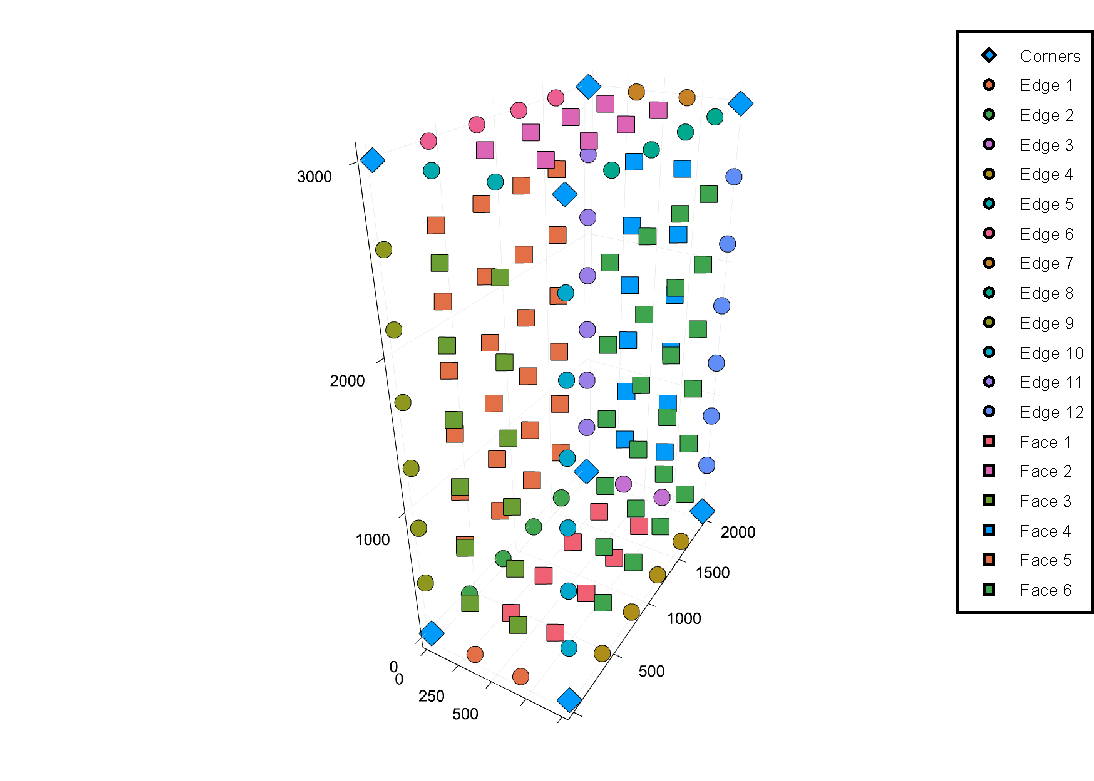
\includegraphics[width=0.8\linewidth]{feNodeSet.pdf}
    \caption[Canonically defined finite element node sets.]{Canonically defined finite element node sets.}
    \label{f:feNodeSet}
\end{figure}

\mintinline{julia}{Julia} has a parametric type are called, \mintinline{julia}{NamedTuple}.
Which are key-value pairs that can be accessed via indices (as one would a tuple), their keys (as one would a dictionary), or dot syntax (as one would a structure).
\begin{minted}[frame=lines]{julia}
julia> d = (a = 1, b = 2 + im, c = false)
(a = 1, b = 2.0 + 1.0im, false)
julia> d[1]
1
julia> d[b]
2.0 + 1.0im
julia> d.c
false
\end{minted}
They act like on-the fly structures and are very convenient when making composable and generic code. The variable \mintinline{julia}{dlnParams}, keeps the drag coefficients in a \mintinline{julia}{NamedTuple}, which can be accessed through the \mintinline{julia}{dragCoeffs} field. This makes swapping mobility functions a breeze without modifying existing source code. \mintinline{julia}{NamedTuples} are also used in the FE mesh data structure, where they represent surface node sets.
\begin{minted}[frame=lines]{julia}
julia> keys(meshC.surfNode)
(:x0y0z0, :x1y0z0, :x1y1z0, :x0y1z0, :x0y0z1, :x1y0z1, 
 :x1y1z1, :x0y1z1, :x_y0z0, :y_x1z0, :x_y1z0, :y_x0z0, 
 :x_y0z1, :y_x1z1, :x_y1z1, :y_x0z1, :z_x0y0, :z_x1y0, 
 :z_x1y1, :z_x0y1, :xz_y0, :yz_x1, :xz_y1, :yz_x0, 
 :xy_z0, :xy_z1)
\end{minted}
The keys say exactly what they represent, and are canonically ordered \cite{femcanonical}. Corners come first (\mintinline{julia}{:x0y0z0}), then edges (\mintinline{julia}{:x_y0z0}), and finally faces (\mintinline{julia}{:xz_y0}), making the creation of different boundary conditions a very easy, self-documenting, literal process.

We can easily generate the boundary conditions for our model, as well as the sparse vectors that will hold the loading information.
\begin{minted}[frame=lines, linenos]{julia}
# Generate boundary conditions and sparse vectors 
# that will hold loading information
boundaryC, forceDispC = Boundaries(femParamsC, meshC)
# Plot boundary conditions
figCBC = plotBoundaries(boundaryC, meshC)
\end{minted}
This uses our canonical definition of the boundary conditions (\cref{f:cantileverNodeSet}), but users can modify them through keyword arguments.
\begin{figure}
    \centering
    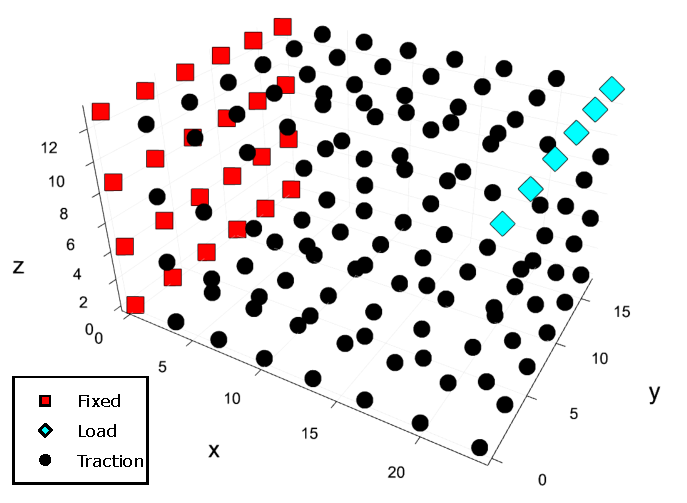
\includegraphics[width=0.6\linewidth]{cantilever.pdf}
    \caption{DDD.jl canonical cantilever loading boundary node sets.}
    \label{f:cantileverNodeSet}
\end{figure}
Through the magic of multiple dispatch, we can also create boundary conditions for pillar loading \cref{f:pillarLoad}. Here we went with a different mesh, but we could just as easily have used the same one as before, as long as the \mintinline{julia}{model} parameter given to the \mintinline{julia}{FEMParameters} is \mintinline{julia}{PillarLoad()}.
\begin{minted}[frame=lines, linenos]{julia}
# Pillar loading
femParamsP = FEMParameters(;
    type = DispatchRegularCuboidMesh(),
    order = LinearElement(),
    model = PillarLoad(),
    dx = 17.0,
    dy = 13.0,
    dz = 23.0,
    mx = 5,
    my = 3,
    mz = 7,
)
meshP = buildMesh(matParams, femParamsP);
boundaryP, forceDispP = Boundaries(femParamsP, meshP);
\end{minted}
\begin{figure}
    \centering
    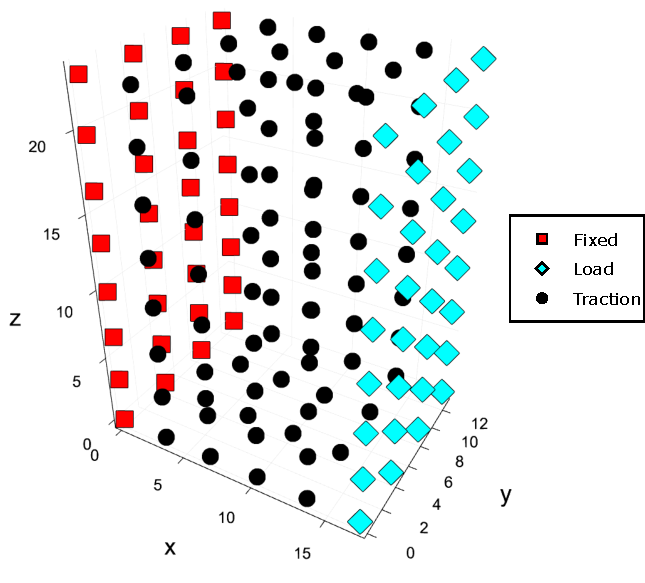
\includegraphics[width=0.6\linewidth]{pillar.pdf}
    \caption{DDD.jl canonical pillar loading boundary node sets.}
    \label{f:pillarLoad}
\end{figure}

\section{Generating dislocations}

Generating dislocation sources is also quite easy. We can use some information from the simulation parameters to generate two types of dislocations,
\begin{inparaenum}
    \item prismatic loop with 8 sides, 8 nodes and 8 segments with $\vec{b} = [1\, 1\, 1]$ and $n = [\overline{1}\, 1\, 0]$,
    \item and a shear loop with 5 sides, 10 nodes and 10 segments with $b = [1\, 1\, \overline{1}]$ and $n = [1\, \overline{1}\, 0]$.
\end{inparaenum}
Both structures represent 5 loops with segment lengths equal to \mintinline{julia}{segLen}, which will generate random uniformly distributed loops in $x = [0,\, dx]$, $y = [0,\, dy]$, $z = [0,\, dz]$.
\begin{minted}[frame=lines, linenos]{julia}
# Julia supports multiple assignments in a single line
# Assign the domain size and length scale for the dislocation
# segments.
dx, dy, dz = femParamsC.dx, femParamsC.dy, femParamsC.dz
segLen = (dlnParams.minSegLen + dlnParams.maxSegLen) / 2

prismOct = DislocationLoop(;
    loopType = loopPrism(), # Prismatic loop
    numSides = 8,   # 8 sides
    nodeSide = 1,   # 1 node per side (corners)
    numLoops = 5,   # Will generate 5 loops in the network
    segLen = segLen * ones(8), # Each side is of equal length
    slipSystemIdx = 1,  # Slipsystem 1
    slipSystem = slipSystems,   # Available slip systems
    label = nodeTypeDln.(ones(Int, 8)), # Node type
    buffer = 0, # Spacing for the distribution, may change in the future
    range = [0 dx; 0 dy; 0 dz], # Range on which to distribute
    dist = Rand(),  # Random uniform distribution in space
)
shearPent = DislocationLoop(;
    loopType = loopShear(), # Shear loop
    numSides = 5,
    nodeSide = 2,   # Two nodes per side (corners and mid-segment)
    numLoops = 5,
    segLen = segLen * ones(10), # 10 segments per loop this time
    slipSystemIdx = 2,
    slipSystem = slipSystems,
    label = nodeTypeDln.(ones(Int, 10)),
    buffer = 0,
    range = [0 dx; 0 dy; 0 dz],
    dist = Rand(),
)
\end{minted}
When the loops are generated, only one of each is made, and they are centred about the origin (\cref{f:templateLoops}). Their purpose is to serve as templates for later use.
\begin{figure}
    \centering
    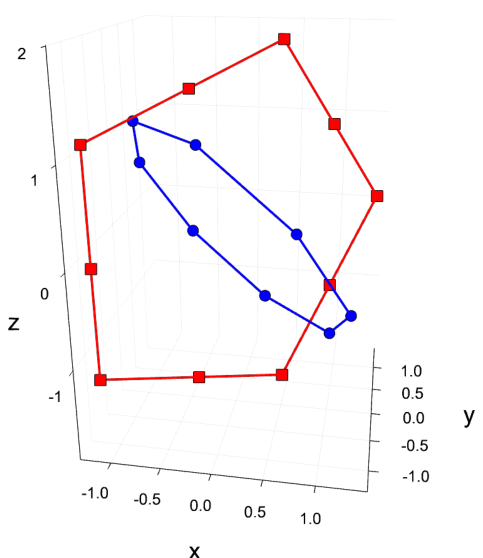
\includegraphics[width=0.6\linewidth]{loops.pdf}
    \caption{Template loops for network generation.}
    \label{f:templateLoops}
\end{figure}
How the loops are distributed is down to the \mintinline{julia}{dist} field, there are currently a zero-distribution (loops centered at the origin), random uniform, and random normal distributions. New ones can be quickly and easily added by subtyping the distribution type and making a function that dispatches on it.\footnote{This can also be achieved with \mintinline{julia}{eval()}, but it is unsafe because \mintinline{julia}{eval()} can execute whatever code it is given.} The loop generation source code does not have to be modified for this to happen.

A nice feature of strongly typed languages is the intrinsic safety they offer via types. One of the ways in which this can be enforced is through the use of enumerated types for categorial variables. In 3D discrete dislocation dynamics we can have different types of nodes with different behaviours. We can safeguard our model against regressions (bugs introduced through further development) and reduce the memory requirements through the use of such types. To find out what they are and represent we can query the documentation for dislocation node type, \mintinline{julia}{nodeTypeDln}.
\begin{minted}[frame=lines]{julia}
julia>?nodeTypeDln
search: nodeTypeDln nodeTypeFE

  @enum nodeTypeDln begin
      noneDln = 0    # Undefined node, value at initialisation
      intMobDln = 1  # Internal mobile node
      intFixDln = 2  # Internal fixed node
      srfMobDln = 3  # Mobile surface node
      srfFixDln = 4  # Fixed surface node
      extDln = 5     # External node
      tmpDln = 6     # Temporary flag, used during topological 
                     # operations
  end 
\end{minted}
Node labels cannot have values other than these, unless the type is expanded, meaning the change has to be deliberate and thought out.

There are multiple ways of generating dislocation networks, but the preferred way is to use the loops already generated. Bespoke networks can be generated manually and developers can leverage multiple dispatch to do create new methods for the \mintinline{julia}{DislocationNetwork} function. Since we have loops that we've already generated, we can create the network from them. The function automatically allocates $N\log_2N$ places for $N$ total nodes and segments in the network, which leaves room for expansion without having to dynamically allocate memory every time a node is created. The topological operations also use this heuristic when the network needs to be expanded beyond its currently allocated memory.\footnote{It does not yet remove excess allocated memory, but will do in the future.}
\begin{minted}[frame=lines, linenos]{julia}
network = DislocationNetwork((prismOct, shearPent))
# Plot network pre-remeshing.
networkFEFig = plotNodes(
    meshC,
    network,
    m = 2,
    l = 3,
    linecolor = :blue,
    markershape = :circle,
    markercolor = :blue,
    legend = false,
    camera = camera = (-15, 25)
)
\end{minted}

\section{Current capabilities}

\Cref{f:networkPrePost} shows the network pre- and post- surface and internal remeshing. The surface remeshing algorithm uses nodal velocities to find where the dislocation would have intersected the volume if it were moving with constant velocity. It also incorporates the correction described in \cref{s:surfRem}.
\begin{minted}[frame=lines, linenos, mathescape]{julia}
# Compute total force on segments = 
# Peach-Koehler force (zero because there is no $\vec{\hat{u}}$)
# + Self force
# + Remote force
calcSegForce!(dlnParams, matParams, meshC, forceDispC, network)
# Compute nodal mobilities
dlnMobility!(dlnParams, matParams, network)
# Remesh the surface
network = remeshSurfaceNetwork!(meshC, boundaryC, network)
# Coarsen the internal network
network = coarsenNetwork!(dlnParams, matParams, meshC, 
                forceDispC, network)
# Refine the internal network
network = refineNetwork!(dlnParams, matParams, meshC, 
                forceDispC, network)
# Plot remeshed network
remFEFig = plotNodes(
    meshC,
    network,
    m = 2,
    l = 3,
    linecolor = :blue,
    markershape = :circle,
    markercolor = :blue,
    legend = false,
    camera = (-15, 25)
)
# Find all surface nodes (both mobile and fixed)
idx = findall(x -> x ∈ (3, 4), network.label)
# Plot surface nodes on the same figure as red circles.
scatter!(network.coord[1, idx], network.coord[2, idx], 
    network.coord[3, idx], m = 2, markercolor = :red)
\end{minted}
\begin{figure}
    \centering
    \begin{subfigure}[t]{0.48\linewidth}
        \centering
        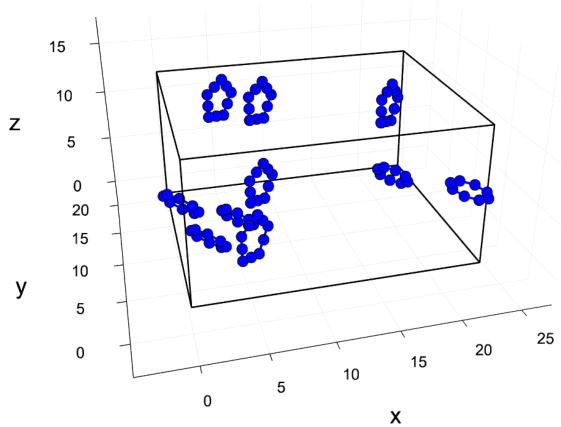
\includegraphics[width=\linewidth]{preremnet.pdf}
        \caption{Pre remeshed network.}
    \end{subfigure}
    ~
    \begin{subfigure}[t]{0.48\linewidth}
        \centering
        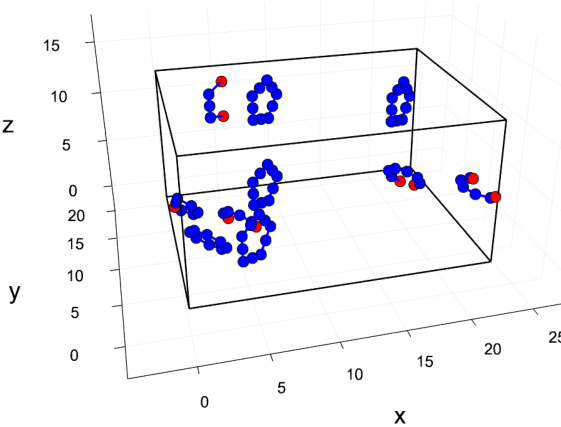
\includegraphics[width=\linewidth]{postremnet.pdf}
        \caption{Post remeshing network.}
    \end{subfigure}
    \caption[Network pre and post remeshing.]{Network pre and post remeshing. The boundary conditions require the $yz$ plane at $x=0$ to be impenetrable to stop a slip step from forming in the surface with fixed displacement boundary conditions as explained in \cref{s:surfRem}.}
    \label{f:networkPrePost}
\end{figure}
The code can also now compute dislocation induced displacements by \citet{bromage2018calculating}, \cref{f:dlnDisp} plots them scaled 20 times.
\begin{minted}[frame=lines, linenos]{julia}
# Dislocation displacements.
calc_uTilde!(forceDispC, meshC, boundaryC, matParams, network)
# Copy structure to another variable.
deformedMesh = deepcopy(meshC)
# Add 20 times the displacements to the dislocation 
# displacement boundaries.
deformedMesh.coord[reshape(boundaryC.uDofsDln, :, 3)'] += 
    20 * forceDispC.uTilde[reshape(boundaryC.uDofsDln, :, 3)']
plotBoundaries(boundaryC, deformedMesh; camera = (-20, 20))
\end{minted}
\begin{figure}
    \centering
    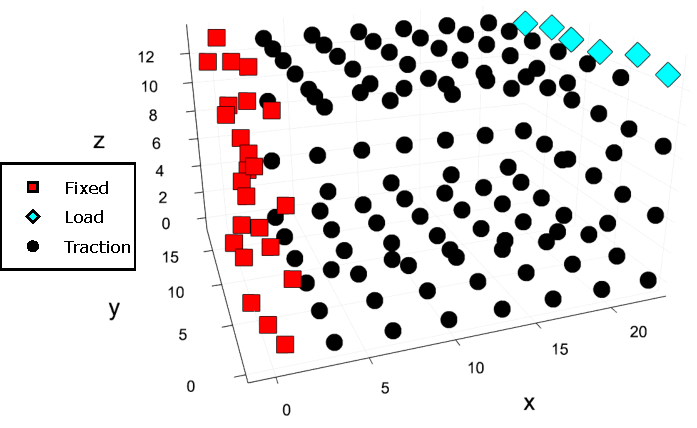
\includegraphics[width=0.6\linewidth]{dispBound.pdf}
    \caption{DDD.jl calculates dislocation induced displacements.}
    \label{f:dlnDisp}
\end{figure}
We're also able to calculate field point stresses (for numeric tractions), detect and resolve collisions, and calculate lazy numeric tractions for a single gauss quadrature point. However, resolving collisions and numeric tractions have not been tested yet.

\section{Performance remarks}

\mintinline{julia}{Julia} was built as a language for scientific computing. Its primary goal is to be high performance, generic, and easy to use. It should come as no surprise that DDD.jl is substantially faster than the \mintinline{matlab}{MATLAB} portions of EasyDD. It is however, somewhat surprising that even C-accelerated portions of EasyDD perform better in DDD.jl and not by an insignificant amount. All the preliminary performance comparisons were done on an AMD Ryzen 7 1700 \@ 3.0 GHz.
\begin{enumerate}
    \item The $\mathcal{O}(N^2)$ remote force computation is 10\% faster than its equivalent \mintinline{c}{C} function. DDD.jl also has a CPU parallelisation. It was almost trivial to implement, which is definitely not the case for \mintinline{c}{C}. For large numbers of dislocation segments ($>500$), it offers linear scaling with number of threads used (at least on the aforementioned processor).
    \item The self-forces and Peach-K\"{o}hler forces as a result of the dislocations being inside a cuboid mesh are both $10\times$ faster than their \mintinline{matlab}{MATLAB} counterparts.
    \item DDD.jl's mesh refinement uses a better heuristic than dynamically sizing arrays every time a new node is added to the network, so it is about as slow as \mintinline{matlab}{MATLAB}'s when it needs to allocate memory. When it does not need to allocate memory, it is $>100\times$ faster. Mesh coarsening is $3\times$ faster.
    \item The calculation of field point stresses for numeric tractions is $30\%$ faster than its \mintinline{c}{C} counterpart.
    \item Building the FE mesh is $>10\times$ faster.
    \item The outdated mobility law is $>30\times$ faster, and has not required dampening the inversion during any tests.
    \item The dislocation-induced displacement calculation is $>10\times$ faster.
    \item The cholesky factorisation of the stiffness matrix for free degrees of freedom is $20\times$ faster and uses a substantially smaller amount of memory.
\end{enumerate}
Collision detection has not yet been compared to its EasyDD counterpart (which is written in \mintinline{c}{C}), and neither have the untested procedures. However, numeric tractions should be substantially faster as the field point stress calculation is faster in DDD.jl, and the DDD.jl version allocates no memory. If the trend holds, the rest of the functions should also see large increases in speed.

The memory footprint is also \emph{much} smaller. Care has been taken to do things as optimally as possible, and \mintinline{julia}{Julia}'s typesystem lets sparse arrays be treated in \emph{exactly} the same way as dense ones, which is not always the case in \mintinline{matlab}{MATLAB}, which has thwarted efforts at sparsifying various arrays that would benefit from it.

The total number of lines of code so far is $\sim 3300$ with many duplicates due to mutating and non-mutating forms of functions\footnote{Mutating functions don't allocate memory, so they tend to be faster.}. Some refactoring of common code should put it at $\sim 1800$ lines, which is about the same number of lines in the remote force calculation written in \mintinline{c}{C}.

Moreover, doing the equivalent of what we have shown on EasyDD requires a substantially larger amount of code and a not insignificant amount of knowledge of its inner workings. From generating the network, to defining values for its parameters---which, despite the fact that EasyDD provides a reasonable set of defaults, users can easily define derived parameters incorrectly and be none the wiser until things break. The barrier to entry and potential for error are quite high. We use the code all the time, and have worked to greatly improve it. Yet we miss things regularly only to catch them after a simulation does something unexpected hours later. Even when everything is in order, seeing whether a simulation is well-callibrated can take hours. Often, multiple iterations of a simulation need to be run to find an appropriate callibration which reproduces an experiment---i.e. tuning the source size, number of sources, slip systems, loading rate, Poisson ratio, etc. Having to wait for hours or days before being able to see whether a simulation is properly callibrated is quite unproductive.

\section{Conclusions and proposal}\label{s:concProp}

What started as a side project to learn and escape from the world during the last year has resulted in quite a promising avenue for future research. One that lets us have our cake and eat it too. Not only is it performant, it is almost trivially parallelisable on both CPUs and GPUs; while staying easy to use and develop. What \mintinline{julia}{Julia} offers is almost incomprehensible. The performance of \mintinline{c}{C} and \mintinline{fortran}{Fortran}; the syntax and interactivity of \mintinline{python}{Python} and \mintinline{r}{R}; metaprogramming of \mintinline{lisp}{Lisp}; and fully integrated testing and package environments of \mintinline{rust}{Rust} and \mintinline{go}{Go}.

A tool is only as good as the craftsman who weilds it. We aspire to be among those elite craftsmen. Why then, should we not use as good a tool as we can? During the course of this project, the whole Tarleton group have made gigantic strides with EasyDD. It has indeed come a \emph{very} long way, but we can do better.

Some issues are so deeply intertwined with how the software was originally designed that they cannot be separated from how it fundamentally operates. To fix them, a fresh new start is needed. Given the extremely encouraging results of what amounts to a pandemic hobby, it seems worthwhile to continue this as a research software engineering project post-DPhil. We think it's better to do so now rather than wait until there is no more juice left to squeeze out of \mintinline{matlab}{MATLAB}. Not only so the shackles of proprietary software can be broken; but also so the full, ambitious vision of EasyDD can be realised.
\savearabiccounter
% 4086 words